\documentclass[border=0pt]{standalone}
\usepackage[T1]{fontenc}
\usepackage{lmodern,amsmath,graphicx,tikz}
\usetikzlibrary{arrows.meta,calc,positioning}
\definecolor{ink}{HTML}{20252C}
\definecolor{blue}{HTML}{0072B2}
\definecolor{raw}{HTML}{C1272D}
\definecolor{green}{HTML}{39775A}
\definecolor{orange}{HTML}{D55E00}
\definecolor{muted}{HTML}{69717A}
\tikzset{every node/.style={font=\fontsize{9}{10.8}\selectfont,text=ink,inner sep=1mm,outer sep=0pt,align=center},
 title/.style={font=\fontsize{9}{10.8}\selectfont\bfseries},
 detail/.style={font=\fontsize{8.5}{10.2}\selectfont,text=muted},
 box/.style={draw=blue!65,fill=blue!3,line width=.65pt,rounded corners=1mm,minimum height=13mm},
 flow/.style={draw=blue,line width=.8pt,shorten <=.5pt,shorten >=.5pt,-{Latex[length=2mm,width=1.3mm]}},
 ref/.style={draw=green,dashed,line width=.7pt}}

\begin{document}
\begin{tikzpicture}[x=1mm,y=1mm]
\path[use as bounding box] (0,0) rectangle (162,84);
\node[title,anchor=west] at (1,80) {(a) Supplied apparatus design};
\node[anchor=south,inner sep=0] at (40,21) {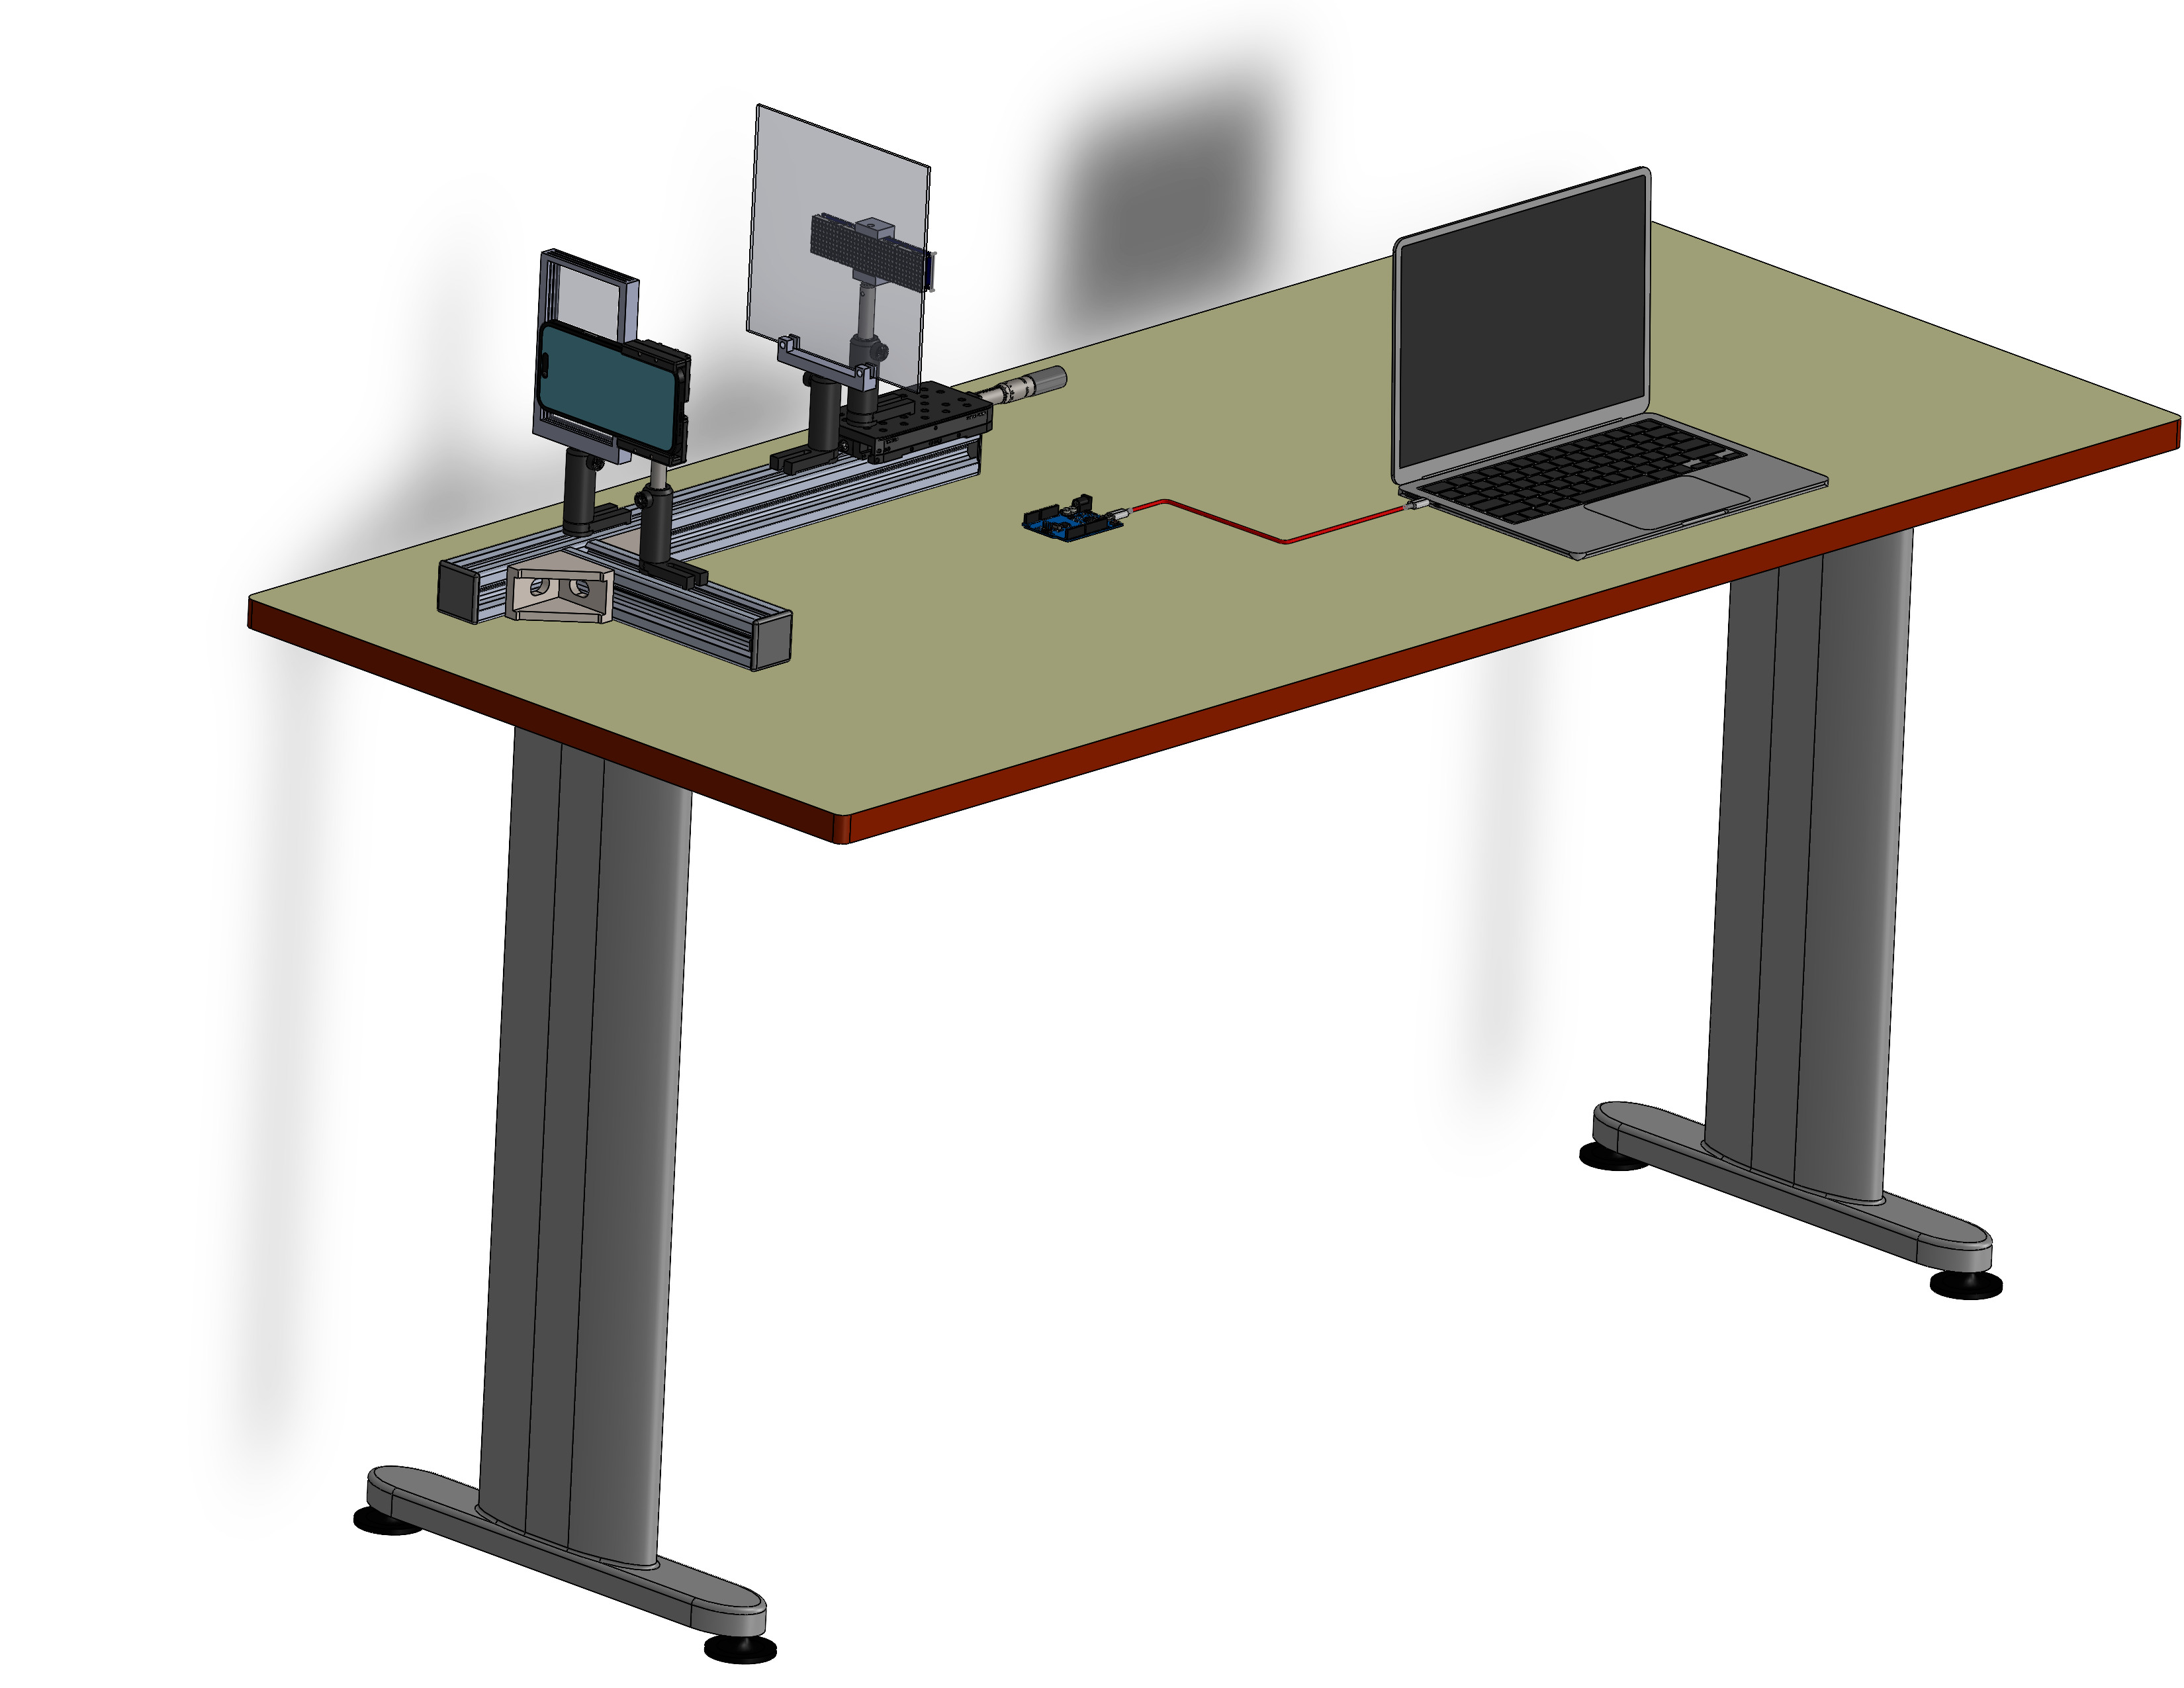
\includegraphics[width=77mm,height=52mm,keepaspectratio]{../reference/Setup_SuperResolution.JPG}};
\node[title,anchor=west] at (83,80) {(b) Optical and data paths};
\draw[muted!25] (81,17)--(81,73);
\draw[green,fill=green!5] (87,46) rectangle (95,63);
\foreach \x in {89,93}\foreach \y in {49,53,57,61}\fill[orange] (\x,\y) circle (.7mm);
\draw[blue!50,fill=blue!8] (112,44) rectangle (115,65);
\draw[ink,fill=ink!5,rounded corners=1mm] (141,48) rectangle (156,61);
\draw[ink,fill=blue!12] (140,54.5) ellipse (2mm and 4mm);
\draw[flow] (97,54.5)--(109,54.5);\draw[flow] (117,54.5)--(136,54.5);
\node[detail] at (92,38) {Blinking\\LED sources};\node[detail] at (115,38) {Diffusive\\screen};\node[detail] at (148,38) {Camera};
\node[box,text width=60mm,minimum height=12mm] (soft) at (120,21) {Video $\rightarrow$ centroid localization\\$\rightarrow$ positions and rendered image};
\draw[flow,draw=orange] (156,54.5)--(159,54.5)--(159,21)--(soft.east);
\node[detail,anchor=west,align=left,text width=155mm] at (1,5) {Conceptual diagram; not to scale.\\Effective blur and object-plane pixel size require calibration.};
\end{tikzpicture}
\end{document}
